\mathchardef\period=\mathcode`.
\documentclass[a4paper]{article}
\usepackage[top=1.45cm, bottom=1cm, left=1cm, right=1cm]{geometry}

\usepackage{parskip} % Package to tweak paragraph skipping
\usepackage{tikz} % Package for drawing
\usepackage{tkz-euclide}
\usepackage{siunitx}
\usepackage{wrapfig}
\usepackage{graphicx}

\usetikzlibrary{fit,positioning}
\usetikzlibrary{arrows.meta}
\usetikzlibrary{patterns,patterns.meta}
\usepackage[inline]{enumitem}
\usepackage{amsmath,amssymb}
\usepackage{tasks}
\usepackage{amsmath}
\usepackage{hyperref}
\usepackage[main=lithuanian, german, shorthands=off]{babel}
\usepackage{tgpagella}
\usepackage[L7x,T1]{fontenc}
\usepackage[utf8]{inputenc}
\usepackage{enumitem}
\usepackage{booktabs} % For better looking tables
\usepackage{venndiagram}
\usepackage{subfig}
\usepackage{multirow}
\usepackage{tabularray}
\usepackage{lipsum}
\usepackage{fancyhdr}

\usepackage{blindtext}
\usepackage{adjustbox}
\AfterEndEnvironment{wrapfigure}{\setlength{\intextsep}{0mm}}

\usepackage{icomma}

% Header | Footer 
\fancyhf{} % clear all header and footer fields
\fancyhead[R]{ funkcijų transformacijos | tiesinės funkcijos | laipsninės
      funkcijos }
% L for Left, you can also use R for Right or C for Center
\fancyfoot[R]{funkcijų transformacijos | tiesinės funkcijos | laipsninės
      funkcijos}

% L for Left, you can also use R for Right or C for Center
\setlength{\headheight}{0.5pt} % Adjust the head height
\renewcommand{\headrulewidth}{0.4pt} % Line under the header
\renewcommand{\footrulewidth}{0.4pt} % Line above the footer
% Header | Footer 

\newcommand{\germanqq}[1]{{\selectlanguage{german}\glqq#1\grqq\selectlanguage{english}}}

\DeclareMathOperator{\tg}{tg}
\newcommand{\tgx}{\tg x}

\DeclareMathOperator{\arctg}{arctg}
\newcommand{\arctgx}{\arctg x}

\makeatletter
\newcommand*{\rom}[1]{\expandafter\@slowromancap\romannumeral #1@}
\makeatother

\title{Savarankiškas darbas nr. 4}
\author{Vilius Paliokas}
\date{2023/02/14}

\setlist{after=\vspace{\baselineskip}}

% Title spacing
\usepackage{titlesec}
\titlespacing*{\subsection}{0pt}{\baselineskip}{0.5\baselineskip}
% ------------------------ 

\begin{document}
\thispagestyle{fancy}

\subsection*{1 variantas}

\begin{enumerate}
      \item (\textit{2 taškai}) Duota funkcija $y=f(x)=50-\frac{1}{2}x$. Kurie iš žemiau pateiktų
            taškų priklauso funkcijai $y=f(x)$ (jeigu tokių taškų nėra,
            parašykite \germanqq{Nei vienas}):

            \begin{tasks}[item-format={\normalfont}, after-item-skip=2mm,
                        label=\Alph*, label-format={\bfseries}](5)
                  \task $(-20; 60)$;
                  \task $(-50; 0)$;
                  \task $(0; 0)$;
                  \task $(0; 50)$;
                  \task $(20; 40)$;
            \end{tasks}
\end{enumerate}
\vspace*{-5mm} % Decrease or increase the -2mm as necessary

\begin{minipage}[t]{0.65\textwidth}
      \vspace*{-50mm} % Decrease or increase the -2mm as necessary
      \begin{enumerate}[itemsep=2mm, parsep=1mm, start=2]
            \item (\textit{2 taškai}) Apibūdinkite funkciją $y=f(x)=3x+2$ (apibrėžimo, reikšmių
                  sritis;
                  funkcijos didėjimo ir mažėjimo intervalai; mažiausia,
                  didžiausia
                  reikšmės; $y>0$, $y<0$, $y=0$, kai \ldots) ir nubraižykite
                  jos
                  grafiką.

            \item (\textit{1 taškas}) Parašykite tiesės funkciją $y=f(x)$, kai šios funkcijos
                  grafikas
                  eina per taškus $A(20; 50)$ ir $B(-10; -10)$.

            \item (\textit{1 taškas}) Parašykite dvi funkcijas $y=g(x)$ ir $y=h(x)$, kurios yra
                  lygiagrečios funkcijai $y=f(x)=-5$.

            \item (\textit{2 taškai}) Nustatykite, ar funkcijos $y=f(x)$ grafikas yra simetrinis
                  $OY$
                  ašies atžvilgiu, ar pradžios taško $(0; 0)$ atžvilgiu, ar nei
                  $OY$
                  ašies atžvilgiu, nei pradžios taško atžvilgiu, kai:

                  \begin{tasks}[item-format={\normalfont},
                              after-item-skip=2mm](3)
                        \task $f(x)=2x^3$;
                        \task $f(x)=-14$;
                        \task $f(x)=2x^2-x$;
                  \end{tasks}

            \item (\textit{2 taškai}) Apibūdinkite funkciją $y=f(x)=2x^2+3$ (apibrėžimo, reikšmių
                  sritis;
                  funkcijos didėjimo ir mažėjimo intervalai; mažiausia,
                  didžiausia
                  reikšmės; $y>0$, $y<0$, $y=0$, kai \ldots).

            \item (\textit{1 taškas}) Parašykite funkcijos $y=g(x)$ reiškinį, kai
                  $f(x)=-\frac{2}{x}$,
                  $g(x)=\frac{1}{2}f(x-2)+1$.

            \item (\textit{1 taškas}) Pavaizduotas funkcijos $y=f(x)$ grafikas (\textit{žiūrėti į 1-ąjį grafiką}). Nubraižykite
                  funkcijos
                  $y=g(x)$, kai $g(x)=-2f(x-1)+3$.

            \item (\textit{papildomas, 1 taškas}) Kodėl pavaizduotas grafikas
                  nėra funkcijos grafikas? (\textit{žiūrėti į 2-ąjį grafiką})
      \end{enumerate}
\end{minipage}
\begin{minipage}[]{0.4\textwidth}
      \centering
      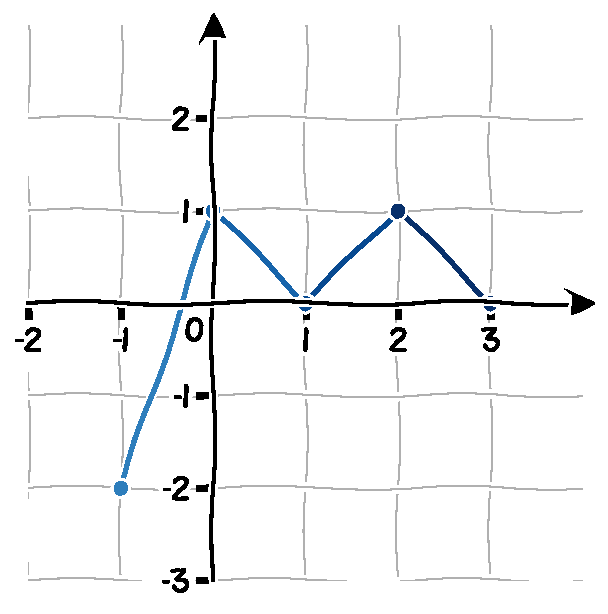
\includegraphics[scale=0.4]{../graph_drawing/f_function_test_1_1.pdf}
      \captionsetup{labelformat=empty}
      \vspace*{-4mm}
      \captionof{figure}{8 užduoties funkcijos grafikas}
      \label{fig:function_example_1}
      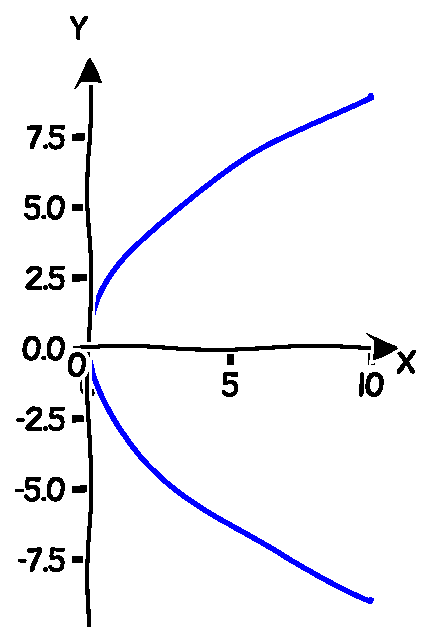
\includegraphics[scale=0.45]{../graph_drawing/sideways_parabola_function_test_1.pdf}
      \captionsetup{labelformat=empty}
      \vspace*{-4mm}
      \captionof{figure}{9 užduoties grafikas}
      \label{fig:function_example_2}
\end{minipage}
\vspace*{-5mm} % Decrease or increase the -2mm as necessary

\subsection*{1 variantas}
\begin{enumerate}
      \item (\textit{2 taškai}) Duota funkcija $y=f(x)=50-\frac{1}{2}x$. Kurie iš žemiau pateiktų
            taškų priklauso funkcijai $y=f(x)$ (jeigu tokių taškų nėra,
            parašykite \germanqq{Nei vienas}):

            \begin{tasks}[item-format={\normalfont}, after-item-skip=2mm,
                        label=\Alph*, label-format={\bfseries}](5)
                  \task $(-20; 60)$;
                  \task $(-50; 0)$;
                  \task $(0; 0)$;
                  \task $(0; 50)$;
                  \task $(20; 40)$;
            \end{tasks}

\end{enumerate}
\vspace*{-5mm} % Decrease or increase the -2mm as necessary

\begin{minipage}[t]{0.65\textwidth}
      \vspace*{-50mm} % Decrease or increase the -2mm as necessary
      \begin{enumerate}[itemsep=2mm, parsep=1mm, start=2]
            \item (\textit{2 taškai}) Apibūdinkite funkciją $y=f(x)=3x+2$ (apibrėžimo, reikšmių
                  sritis;
                  funkcijos didėjimo ir mažėjimo intervalai; mažiausia,
                  didžiausia
                  reikšmės; $y>0$, $y<0$, $y=0$, kai \ldots) ir nubraižykite
                  jos
                  grafiką.

            \item (\textit{1 taškas}) Parašykite tiesės funkciją $y=f(x)$, kai šios funkcijos
                  grafikas
                  eina per taškus $A(20; 50)$ ir $B(-10; -10)$.

            \item (\textit{1 taškas}) Parašykite dvi funkcijas $y=g(x)$ ir $y=h(x)$, kurios yra
                  lygiagrečios funkcijai $y=f(x)=-5$.

            \item (\textit{2 taškai}) Nustatykite, ar funkcijos $y=f(x)$ grafikas yra simetrinis
                  $OY$
                  ašies atžvilgiu, ar pradžios taško $(0; 0)$ atžvilgiu, ar nei
                  $OY$
                  ašies atžvilgiu, nei pradžios taško atžvilgiu, kai:

                  \begin{tasks}[item-format={\normalfont},
                              after-item-skip=2mm](3)
                        \task $f(x)=2x^3$;
                        \task $f(x)=-14$;
                        \task $f(x)=2x^2-x$;
                  \end{tasks}

            \item (\textit{2 taškai}) Apibūdinkite funkciją $y=f(x)=2x^2+3$ (apibrėžimo, reikšmių
                  sritis;
                  funkcijos didėjimo ir mažėjimo intervalai; mažiausia,
                  didžiausia
                  reikšmės; $y>0$, $y<0$, $y=0$, kai \ldots).

            \item (\textit{1 taškas}) Parašykite funkcijos $y=g(x)$ reiškinį, kai
                  $f(x)=-\frac{2}{x}$,
                  $g(x)=\frac{1}{2}f(x-2)+1$.

            \item (\textit{1 taškas}) Pavaizduotas funkcijos $y=f(x)$ grafikas (\textit{žiūrėti į 1-ąjį grafiką}). Nubraižykite
                  funkcijos
                  $y=g(x)$, kai $g(x)=-2f(x-1)+3$.

            \item (\textit{papildomas, 1 taškas}) Kodėl pavaizduotas grafikas
                  nėra funkcijos grafikas? (\textit{žiūrėti į 2-ąjį grafiką})
      \end{enumerate}
\end{minipage}
\begin{minipage}[]{0.4\textwidth}
      \centering
      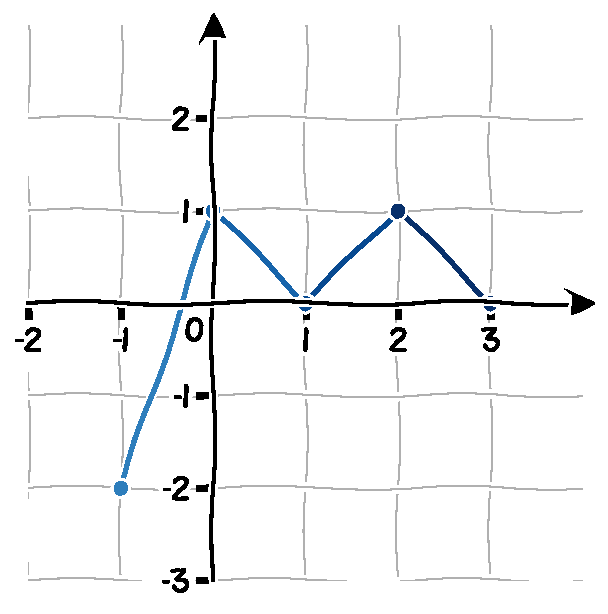
\includegraphics[scale=0.4]{../graph_drawing/f_function_test_1_1.pdf}
      \captionsetup{labelformat=empty}
      \vspace*{-4mm}
      \captionof{figure}{8 užduoties funkcijos grafikas}
      \label{fig:function_example_1}
      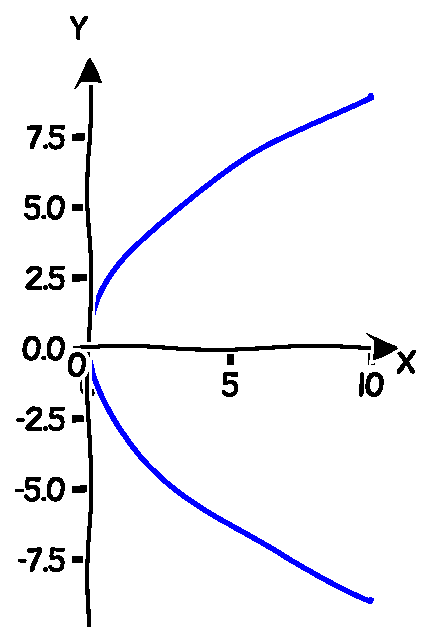
\includegraphics[scale=0.45]{../graph_drawing/sideways_parabola_function_test_1.pdf}
      \captionsetup{labelformat=empty}
      \vspace*{-4mm}
      \captionof{figure}{9 užduoties grafikas}
      \label{fig:function_example_2}
\end{minipage}

\end{document}